\chapter{Background Information}

\section{Sanitization}
Sanitization is the process of removing sensitive information from a document or other message or sometimes encrypting messages, so that the document may be distributed to a broader audience. Sometimes sanitization can be called as an operation that ensures that user input can be safely used in an SQL query. Web applications use malicious input as part of a sensitive operation without having properly checked or sanitized the input values from the user. Previous research on vulneribility analysis has mostly focused on identifying cases which web applications directly uses external input for critical operations. It is suggested that always use proper sanitization method to validate external input values from the user for any application.For example, user inputs must always flow through a sanitizing function before flowing into a SQL query or HTML, to avoid SQL injection or cross-site scripting vulnerabilities.\\

Reflection of security breaches are very significant for high assurance system. For examples of this type of systems are aircraft navigation, where a fault could lead to a crash, various control systems which has critical infrastructure , where an error 
could cause toxic waste to leak, and weapons targeting, where an inaccuracy could result in severe collateral damage. In such
operational environments, the impact is virtually irreversible and must therefore be prevented even if it is likely to occur
with low probability.It's always good that transforming information to a form which is suitable for release or sanitize the information by redacting some portions of it.\\

Some basic purpose of sanitization are given below:
\begin{itemize}
	\item Remove malicious elements from the input.
	\item To identify the set of parameters and global variables which must be sanitized before calling functions.
	\item It is acceptable to first pass the untrusted user input through a trusted sanitization function.	
	\item Any user input data must flow through a sanitization function before it flows into a SQL query.
	\item Confidential data needs to be cleansed to avoid information leaks.
	\item Most paths that go from a source to a sink pass through a sanitizer.
	\item Developers typically define a small number of sanitization functions in libraries.
\end{itemize}

\section{Declassification}
Information security has a challenge to address: enabling information flow controls with expressive information release (or declassification) policies. In a scenario of systems that operate on data with different sensitivity levels, the goal is to provide security assurance via restricting the information flow within the system. Practical security-typed languages support some form of declassification through which high-security information is allowed to flow to a low-security system or observer.\\

To declassify information means lowering the security classification of selected information. Sabelfeld and Sands \cite{ref_3_sabelfeld2009declassification} identify four different dimensions of declassification, what is declassified, who is able to declassify, where the declassification occurs and when the declassification takes place.\\

Myers and Liskov introduced the decentralized label model \cite{ref_4_myers2000protecting}, describing how labels could be applied
to a programming language and then used to check information
flow policy compliance in distributed systems. The framework
includes a declassify function for downgrading data if the
owners policies allow. The model allows principals to define their own downgrading policies.\\


\section{Authentication}
Authentication is the mechanism which confirms the identity of users trying to access a system. For a user to be granted access to a resource, they must first prove that they are who they claim to be. Generally this is handled by passing a key with each request (often called an access token, User verification using user id and password). The system or server verifies that the access token or user id and password is genuine, that the user does indeed have the required privileges to access the requested resource and only then the request granted.\\
Also authentication can be defined as it is the process by which the system validates a user's logon information. A user's name and password are compared to an authorized list and if the system detects a match then access is granted to the extent specified in the permission list for that user.\\

One familiar use of authentication and authorization is access control. A computer system that is supposed to be used only by those authorized must attempt to detect and exclude the unauthorized. Common examples of access control involving authentication include:
\begin{itemize}	
	\item A computer program using a blind credential to authenticate to another program.
	\item Logging in to a computer.	
	\item Using an Internet banking system.
	\item Withdrawing cash from an ATM and more
\end{itemize}

\section{ Detecting Information Flow Errors During Design:}
If a step of function call like authentication, sanitization or declassification is missing inside the program then this can lead to software vulnerabilities.
\begin{figure}[htbp]
	\centering
	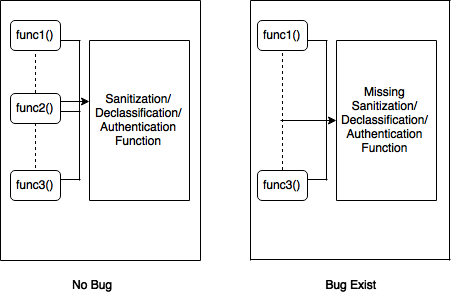
\includegraphics{styles/FunctionCallMissing.png}
	\caption{Information flow errors during design}
\end{figure}


\section{ Detecting Information Flow Errors During Coding:}

